\documentclass[12pt]{article}
\usepackage[utf8]{inputenc}
\usepackage[pdftex]{graphicx}
\usepackage{graphicx}
\usepackage{geometry}
\usepackage{indentfirst}
\usepackage{setspace}
\usepackage{anysize}
\usepackage{makeidx}
\usepackage[brazil]{babel}
\usepackage{longtable}
\usepackage{multirow} 
\usepackage{hyperref}
\usepackage{subfig}
\makeindex

\newcommand{\longtableendfoot}{Continuará na próxima página}

\geometry{
	verbose,
	a4paper,
	left = 30mm,
	top = 30mm,
	right = 20mm,
	bottom = 20mm
}

\begin{document}

\begin{figure}
    \centering
    
\includegraphics[width=16cm]{fga.jpg}
\end{figure}

\begin{titlepage}
% \doublespacing
\centering

\normalfont


\vspace{0.1\textheight}
\vbox{\normalfont{UNB - UNIVERSIDADE DE BRASÍLIA\\CAMPUS GAMA}}
\large{Universidade de Brasília - UnB Gama\\}
\vspace{3cm}


\vbox{\Huge
%Nome do Trabalho
GamePlay

%\ver

\vspace{0.03\textheight}
\hrule }

\vbox{
%Nome da Matéria
Introdução à Computação Gráfica
}
\vspace{0.2\textheight}
%Nomes
\vbox{\scshape
{}
  Developers: Elmar Roberto, Daniel Moura e Eduardo Gomes
  }
\vspace{0.2cm}
{}
\centering
elmarunb@gmail.com | danmoura17@gmail.com | eduardoqgomes@gmail.com \\
\vspace{0.2\textheight}
Brasília, DF~-~\the\year
\end{titlepage}

\onehalfspacing
\tableofcontents
\newpage

\part{Conceito}
\section{Objetivo do Jogo}

O jogo consiste em uma competição do gênero corrida, o jogador terá que capturar “nitros” (pequenos combustíveis para a locomoção do carro) ao longo do percurso, que possibilitam o carro correr. É um jogo que se passa em uma estrada baseada no mundo real com características definidas como objetos coletáveis e manter-se na pista. Os usuários terão suas voltas atualizadas em rankings para então comparar com amigos e demais jogadores. O objetivo principal é fazer o menor tempo correndo no percurso ou coletar a maior quantidade de pontos. No caso do projeto, será apenas uma fase.


\section{Principais características}

\begin{table}[h]
		\caption{Características}
	\begin{center}
	\begin{tabular}{|l|ll|}
		\hline Manter carrinho no percurso \\
		\hline Terminar a fase \\
		\hline Bater rank de melhor tempo e de pontos \\
		\hline Coletar objetos para ganhar pontos \\
		\hline Coletar nitros para reabastecer o carro \\
		\hline Usuário acelera, freia e vira o carro \\
		\hline Jogo do genêro corrida\\
		\hline Simulação \\
		\hline Gráfico 3D \\
		\hline Controle do veículo realizado pelo teclado e mouse \\
		\hline
	\end{tabular}
	\end{center}
\end{table}
\pagebreak
\part{História do Jogo}

\section{Como e aonde começa o jogo}

O jogo não possue uma grande história tomando como base que a finalidade dele é apenas passar a fase imposta. O jogo inicia com o carro centralizado na pista atrás da linha de partida, o jogador tem que esperar o tempo regressivo de 3 segundos acabar para começar a correr.

\section{Cenários do jogo e suas inter-relações}

A ideia geral do jogo seria ir passando das fases tendo uma sequência de paisagens, por conta das restrições de tempo, base e conhecimento, a ideia central é, com o auxílio do Blender, Unity e as linguagens, fazer apenas uma fase. A fase \'e um cen\'ario com montanhas, \'arvores, grama verde e uma cachoeira em um lugar isolado.

O modelo de cen\'ario ser\'a parececido com o modelo teste deste v\'ideo,  \href{https://www.youtube.com/watch?v=9V2GcBU732g}{YouTube}.

\section{Troca de cen\'arios}

Como o jogo em quest\~ao ter\'a apenas uma fase, não haverá troca de cenário.

\section{Final do Jogo}

Ao final da fase, terá uma bandeira de linha de chegada. Quando o jogador chegar a linha, o jogo encerra mostrando ao usu\'ario uma tabela com as informações de tempo de corrida, sua colocação no rank principal e uma opção de voltar a tela inicial e outra de reiniciar a corrida.

\begin{figure}[!h]
	\centering
		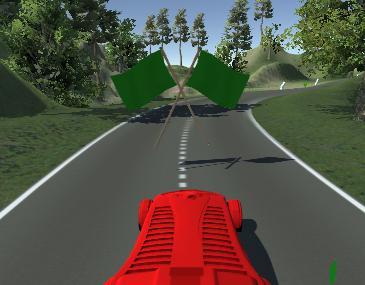
\includegraphics[scale=0.5]{figuras/final}
	\caption{Imagem da tela final}
\end{figure}

\section{Como chegar ao final}

O jogador terá que passar por toda a fase realizando as ações impostas que são: coletar os nitros não deixando o combustível acabar e se mantendo dentro do percurso. Ao chegar na linha de chegada, o jogo encerra.
\pagebreak
\label{2}
\part{Controles}
\section{Movimentos à disposição}

Dentro do jogo o usuário terá movimentos obtidos quanto do teclado e quanto do mouse que servem para jogabilidade e navegar entre as telas do jogo.

\subsection{Teclado}

O jogador terá a sua disposição o usos das teclas 'r' para reiniciar o jogo, a tecla 'c' para continuar em determinadas telas e mais as teclas da imagem abaixo.

\label{teclas}
\begin{figure}[h]
	\centering
	\caption{Imagem ilustrativa das rela\c{c}\~oes das teclas com o carro}
		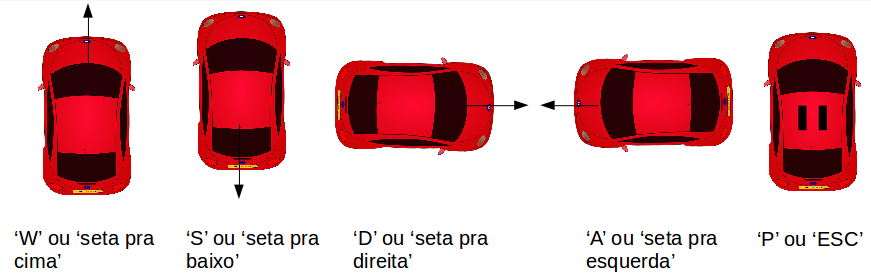
\includegraphics[keepaspectratio=true,scale=0.5]{figuras/movimentos}
\end{figure}

\subsection{Mouse}

O mouse será o meio usado para a movimentação da câmera de jogo.

\pagebreak
\part{Requisitos Tecnol\'ogicos}
\section{Ferramentas de Codificação}

A game engine será a Unity3D que possuem suporte para multiplataforma, altamente otimizado, realiza renderizações e uma das características mais chamativas é que o Unity aceita três linguagens de programção, Boo, JavaScript e C\#, onde o C\# ser\'a usado como a linguagem de script para o projeto por ser bem parecido com o C e C++, facilitando assim o andamento da criação do jogo, pois os desenvolvedores j\'a possuem conhecimentos pr\'evios sobre as linguagens citadas. Os c\'odigos ser\~ao feitos dentro da própria game engine.


\section{Ferramentas de Modelagem}

A ferramenta para construir as cenas fazendo toda a modelagem 3D, também será o Unity3D. \'E um programa de f\'acil manipula\c{c}\~ao, devolve resultados extramente satisfat\'orios, bom sistema de anima\c{c}\~ao e o mais importante para o projeto é que existem vários pacotes prontos de cenas, objetos, personagens etc, disponíveis para uso.

\begin{figure}[!h]
	\centering
		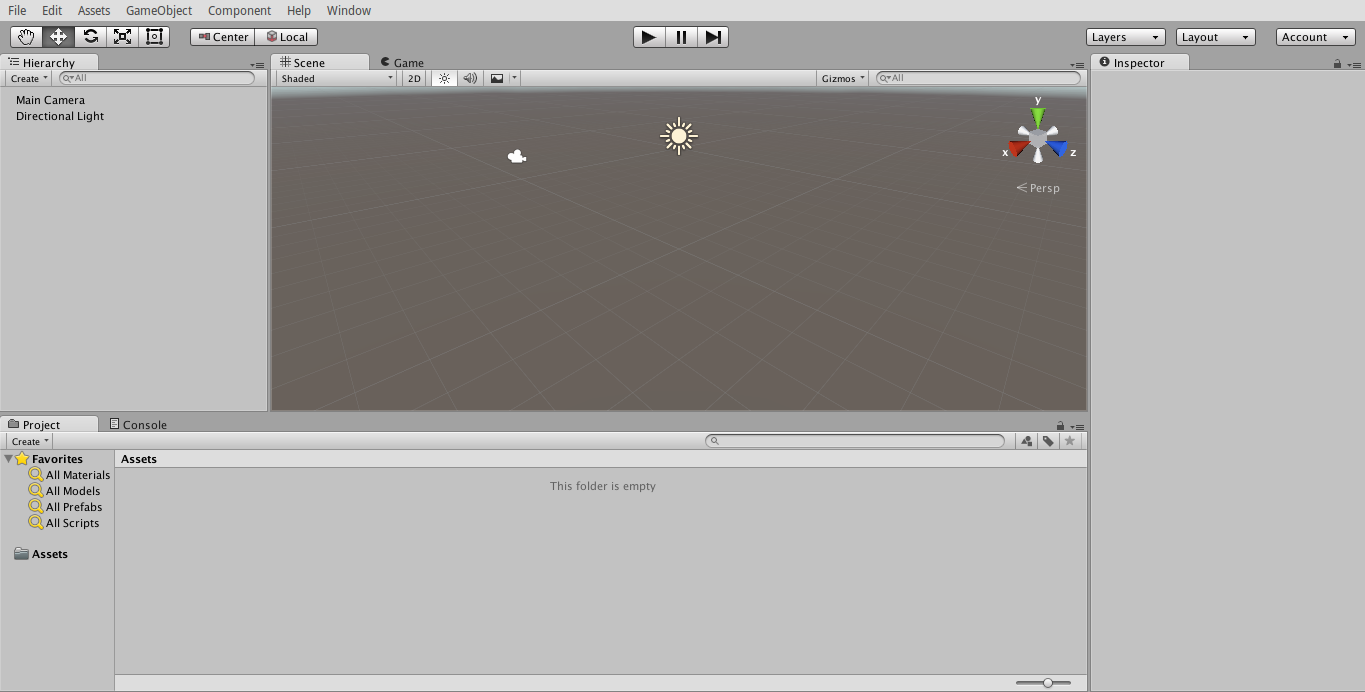
\includegraphics[scale=0.3]{figuras/unity}
	\caption{Interface Unity 3D}
\end{figure}
\pagebreak
\part{Front End}

Assim que o jogo iniciar, ser\~ao mostradas ao usu\'ario quatro telas antes do menu geral do jogo, sendo elas, respectivamente, tela com o logotipo da empresa que no caso também é o logotipo do jogo, tela com o logotipo das tecnologias utilizadas na constru\c{c}\~ao do projeto, Linux, Unity3D e GitHub, tela indicando a classificação indicativa do jogo que no caso \'e livre para todos os públicos e idade e a tela com o simbolo do copyright, em todas as telas as imagens se encontrarão centralizados em fundo preto.

\begin{figure}[!h]
	\centering
		
\includegraphics[keepaspectratio=true,scale=0.4]{figuras/logo}
	\caption{Logotipo da empresa}
\end{figure}

\begin{figure}[!h]
	\centering
	\subfloat[GitHub]{
		
\includegraphics[height=5cm]{figuras/git}
	}
	\quad
	\subfloat[Unity 3D]{
		
\includegraphics[height=5cm]{figuras/unity_logo}
	}
	\quad
	\subfloat[Linux]{
		
\includegraphics[height=5cm]{figuras/linux}
	}
	\caption{Tecnologias}
\end{figure}

\begin{figure}[!h]
	\centering
		
\includegraphics[keepaspectratio=true,scale=0.6]{figuras/indicativa}
	\caption{Faixa indicativa}
\end{figure}

\begin{figure}[!h]
	\centering
		
\includegraphics[keepaspectratio=true,scale=0.4]{figuras/copyright}
	\caption{Copyright}
\end{figure}
\pagebreak
\part{Telas}

\section{Tela de Abertura}

\begin{enumerate}

\item Lista das opções para o jogador \\\\
O jogador terá na tela inicial as opções de iniciar o jogo e vizualizar a tela de créditos. \\

\item Interface com a tela \\\\
Todas as telas terão alguma relação sistema-usuário, algumas por meio do teclado e outras por meio do mouse. \\

\item Modo de salvar e/ou carregar um arquivo de progresso \\\\
No jogo não terá um modo de salvar progresso consequentemente não haverá também a modo de carregar um arquivo de progresso pois o jogo é muito curto não havendo a necessidade dessas funcionalidades, então caso o jogador queira sair no meio da fase, ele perderá todo seu progresso até o momento. \\

\item Músicas \\\\
Serão implementados no jogo três músicas, uma tocará no menu, uma na corrida e a última na tela de game over.

Na questão do gráfico, não se sabe ainda qual será o nível gráfico do jogo então ainda não é possível ter noção se o usuário terá a opção de aumentar ou diminuir essa característica. \\

\end{enumerate}

\label{1}
\begin{figure}[!h]
	\centering
		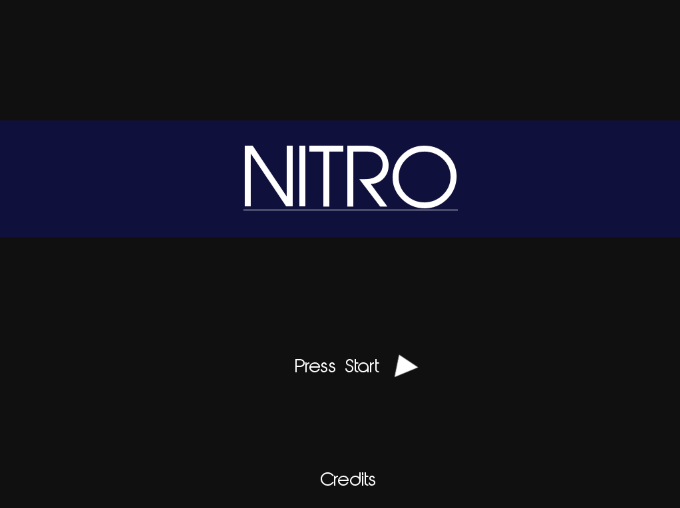
\includegraphics[scale=0.3]{figuras/tela_inicial}
	\caption{Imagem da tela inicial}
\end{figure}

\section{Outras telas}

\subsection{Tela de Créditos}

A tela de créditos aparecerá quando o jogador conseguir ganhar o jogo e se a opção no menu inicial for selecionada, nela passarão os nomes dos desenvolvedores, da materia e da universidade. \\\\\\\\\\

\begin{figure}[!h]
	\centering
		
\includegraphics[scale=0.3]{figuras/creditos}
	\caption{Imagem da tela de créditos}
\end{figure}

\subsection{Tela de Game Over}

A tela de game over irá aparecer caso acabe a gasolina ou o carro saia da pista. \\

\begin{figure}[!h]
	\centering
		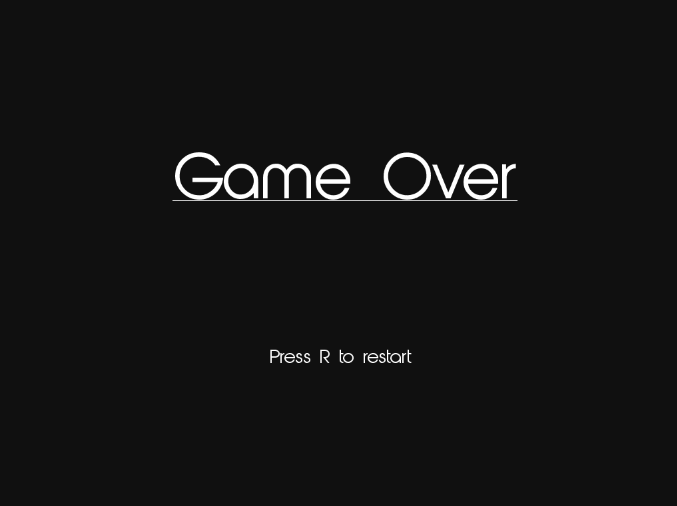
\includegraphics[scale=0.3]{figuras/game_over}
	\caption{Imagem da tela de Game Over}
\end{figure}

\subsection{Tela de Jogo}

\begin{figure}[!h]
	\centering
		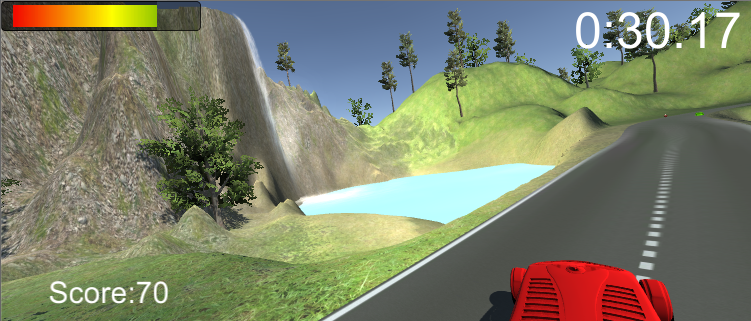
\includegraphics[scale=0.4]{figuras/tela_jogo}
	\caption{Imagem da tela de Jogo}
\end{figure}
\pagebreak
\part{Câmera e HUD}

\section{Câmera}

    A câmera do jogo será movimentada de acordo com a movimentação do mouse, de maneira que ao decorrer do percurso, o carro será mantido centralizado na tela, ou seja, passando a ser uma visão em terceira pessoa em diagonal.

\section{HUD}

    \subsection{Vida}

        Será disponibilizado uma vida ao jogador para cada tentativa não havendo nenhum tipo de energia. O jogador saiu da pista ou a gasolina acabou, a corrida esta encerrada.

    \subsection{Pontuação e Rankings}

        Para cada objeto coletado em jogo, o jogador sera bonificado com a pontuação definida na tabela do documento de visão. Ao final de cada percurso, o sistema fará a totalização da pontuação adquirida ao longo de toda da corrida e guardará o tempo totalizado marcado pelo jogador, para então realizar a atualização desses números na tabela de ranking local do sistema. Terão duas tabelas, a primeira será construida com base nos melhores tempos realizados naquela máquina e a segunda será por pontuação adquirida em jogo, e disposição dos nomes dos jogadores nas tabelas será do menor tempo para o maior e da maior pontuação para a menor. A pontuação será mostrada na parte inferior no canto esquerdo da tela.
        
    \subsection{Combustível}

        A barra de combustível do veículo ficará parte superior à esquerda na tela para que o jogador tenha noção da quantidade que resta para perder a tentativa. Ela será um barra horizontal divida em 3 secções onde quanto mais cheia, ela fica mais esverdeada e quanto mais vazia, ela fica avermelhada.

    \subsection{Tempo}

        O tempo de jogo será baseado no tempo que o jogador permanecer em corrida, enquanto ele se mantiver na pista entre a linha de chegada e a linha de partida, o jogo permanecerá rodando o relógio no canto superior direito.

    \subsection{Medidor de velocidade}

        Na tela da corrida haverá um medidor de velocidade parte inferior à direita na tela. \\\
        
\begin{figure}[!h]
		\centering
	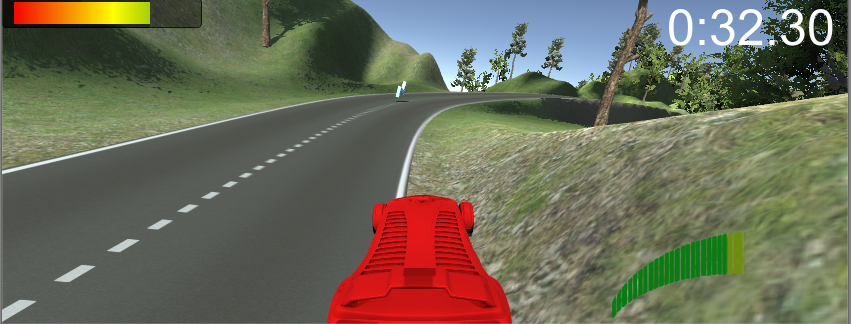
\includegraphics[scale=0.5]{figuras/hud}
		\caption{Tela de jogo}
\end{figure}

	\subsection{Mapa do Jogo}
	
\begin{figure}[!h]
		\centering
	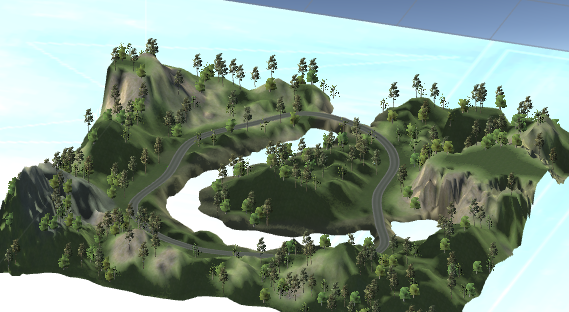
\includegraphics[scale=0.5]{figuras/mapa}
		\caption{Mapa geral do jogo}
\end{figure}	
\pagebreak
\part{Personagem Principal - Veículo}

\section{Descrição}

	O personagem principal do jogo será basicamente o carro utilizado, nunca será visto um piloto então não haverá simulações de personagens humanos.

\begin{figure}[!h]
		\centering
	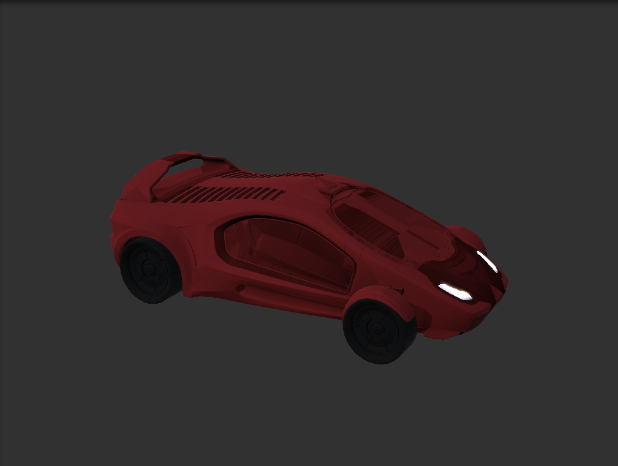
\includegraphics[scale=0.5]{figuras/carro}
		\caption{Imagem do carro de jogo}
\end{figure}
	
\section{Atributos}

	\begin{enumerate}
	
		\item O carro será construido tomando como base o ambiente externo ao percurso, procurando ser realista com base nas proporções do mundo real. 
		\item A movimentação será medida com base no medidor em barras.
		\item Haverá coleta de itens para pontuação, onde acontecerá ao primeiro contato com o carro.
		\item Não haverá danos, onde o carro batendo ou saindo da pista, a corrida encerra.
		\item Comandos para o carro: \hyperlink{teclas}{link}
		\item O carro pode andar apenas dentro da pista
	
	\end{enumerate}
\pagebreak
\part{Power Ups}

\section{Nitro}

\begin{enumerate}

\begin{figure}[!h]
		\centering
	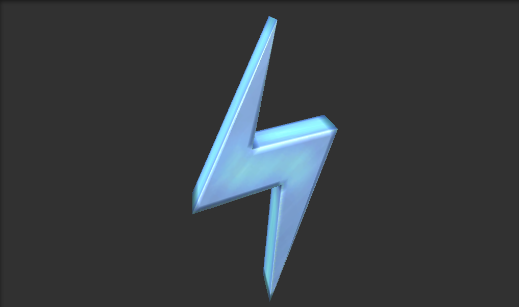
\includegraphics[scale=0.5]{figuras/nitro}
		\caption{Imagem do nitro que abastece o carro}
\end{figure}

	\item Descrição: Este item é o principal do jogo, ele será encontrado no formato de raio em vários pontos ao longo da corrida. Se encontrarão espalhados ao longo do percurso a determinadas distâncias onde terão a função de reabastecer o veículo para prosseguir o jogo.
	\item Formato: Será um objeto azul no formato de raio.
	\item Efeitos: Se o combustível chegar ao fim, a corrida encerra.
	
\end{enumerate}
\pagebreak
\part{Saúde}

\section{Aspectos gerais}

\begin{enumerate}

	\item A quantidade de combustível pode ser considerada um tipo de saúde, pois ela chegando ao fim, o jogo se encerra. Essa barra será mostrada de acordo com a parte de HUD desse documento.
	\item Para recuperar ou preencher essa barra, o jogador deverá realizar a coleta de nitros.
	\item O nitro é considerado um power-up.
	
\end{enumerate}

\section{Vidas e Morte}

\begin{enumerate}

	\item O jogador terá apenas uma vida por jogada.
	\item Ele poderá morrer saindo do percurso ou deixando a gasolina acabar.
	\item Como a corrida é curta, não haverá checkpoints e nem opções de "save/load"

\end{enumerate}

\pagebreak
\part{Pontuação}

\begin{table}[h]
		\centering
		\caption{Ganho de pontos}
	\begin{center}
	\begin{tabular}{|l|l|}
		\hline
			Pontos & Critérios \\ % Note a separação de col. e a quebra de linhas
	
		\hline                               % para uma linha horizontal
			(100*Nível atual) pontos & Nível completo \\
		\hline	10 pontos & Coletar estrela \\
		\hline	15 pontos & Coletar cubo \\
		\hline	20 pontos & Coletar bola \\
		\hline
 
	\end{tabular}
	\end{center}
\end{table}

\begin{figure}[!h]
	\centering
	\subfloat[Estrela]{
		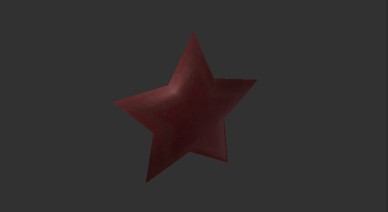
\includegraphics[height=3.5cm]{figuras/estrela}
	}
	\quad
	\subfloat[Cubo]{
		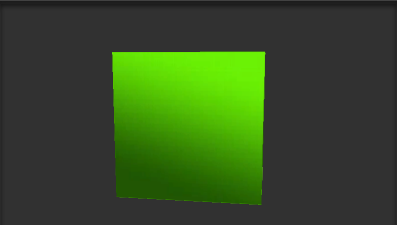
\includegraphics[height=3.5cm]{figuras/cubo}
	}
	\quad
	\subfloat[Bola]{
		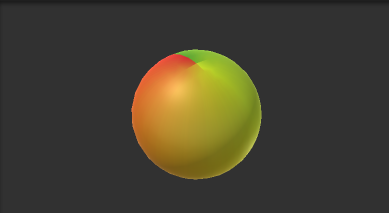
\includegraphics[height=3.5cm]{figuras/bola}
	}
	\caption{Objetos para pontuação}
\end{figure}

\begin{table}[h]
		\centering
		\caption{Perda do jogo}
	\begin{center}
	\begin{tabular}{|l|l|}
		\hline
			Pontos & Critérios \\ % Note a separação de col. e a quebra de linhas
	
		\hline Fim da corrida & Sair da pista \\
		\hline
 
	\end{tabular}
	\end{center}
\end{table}
\pagebreak

\end{document}